\documentclass[a4paper, 12pt]{article}
% math symbols
\usepackage{amssymb}
\usepackage{amsmath}
\usepackage{mathrsfs}
\usepackage{physsummer}


\usepackage{enumitem}
\usepackage[margin = 2cm]{geometry}

\tolerance = 1000
\emergencystretch = 0.74cm



\pagestyle{empty}
\parindent = 0mm

\begin{document}

\setphysstyle{ГЦФО}{Первый тренировочный тур, 9 класс}{02.10.2016}

\subsection*{Задача 1. Двойной мост}

В электрической цепи, схема которой приведена на
рисунке~\ref{fig:2009_09_3}), напряжение между зажимами $C$ и $D$
равно $U_{CD}=15$~В. Известно, что $R\gg r$.

1. Определите показание идеального вольтметра, подключенного к клеммам
$A$ и $B$.

2. Предположим, что к клеммам $A$ и $B$ подключен идеальный
амперметр. Укажите направление тока, идущего через каждый из
резисторов и амперметр.

\sidebyside{2009_09_3}{0.3}{2009_09_4}{0.4}

\subsection*{Задача 2. Старый график}
%\wrapfigcap{2009_09_4}{0.35}

В архивах экспериментатора Глюка нашли график
(рис.~\ref{fig:2009_09_4}) изменения со временем проекции на
вертикальную ось скорости шарика, который был выпущен из
пневматического пистолета вертикально вверх с балкона 17
этажа. Масштаб на оси скорости от времени выцвел, а на оси времени
частично сохранился. Определите начальную скорость шарика и скорость,
с которой шарик упал на землю. Ветра в день эксперимента не было.
% Рег-2009, 9 класс

\subsection*{Задача 3. Вода и масло}

\wrapfigcap{2009_09_5}{0.25}

Два стакана высотой $4H$ заполнены до уровня $3H$ водой и маслом
соответственно (рис.~\ref{fig:2009_09_5}). Плотность воды
$\rho_0 = 10^3$~кг/см$^3$, а плотность масла
$\rho\ruindex{м} = 0{,}8 \cdot 10^3$~кг/см$^3$. Сверху стаканы
соединены заполненной водой тонкой трубочкой с краном. Открытые концы
трубки погружены на $2H$ в каждую из жидкостей. Какие уровни
установятся в стаканах, если кран открыть?
% Рег-2009, 9 класс

\clearpage

\subsection*{Задача 4. Бревно на привязи}
\wrapfigcap{2009_09_1}{0.3}

Подъемный кран медленно поднимает с помощью троса плавающее в воде
бревно (рис.~\ref{fig:2009_09_1}). Трос прикреплен к одному концу
бревна, которое можно считать тонким цилиндром с постоянной
плотностью. Масса бревна --- $m$, длина --- $L$. Отношение плотностей
воды и древесины $\gamma=4/3$. Ускорение свободного падения $g$.

1. Какую минимальную работу $A$ нужно совершить крану, чтобы полностью
вытащить бревно из воды?

2. Постройте график зависимости силы натяжения $T$ троса от высота над
водой $h$ приподнимаемого конца бревна. Укажите характерные точки
графика.

3. Какую работу $A_h$ совершит кран при переводе бревна из одного
наклонного положения в другое наклонное положение, в котором конец
бревна поднялся на высоту $\Delta h=L/5$?
% Рос-2009, 9 класс


\subsection*{Задача 5. <<Дозаправка>> чайника}

Теоретик Баг решил попить чайку. Он взял теплоизолированный чайник,
снабженный миниатюрным термометром, и включил его в электрическую
сеть. Термометр показывал температуру $t_0=20^\circ$C. Через время
$\tau_1=1$~мин, когда вода нагрелась до $t_1=40^\circ$C, он стал
доливать в чайник воду. В момент $\tau_2=3{,}5$~мин, когда температура
воды достигла $t_2=50^\circ$C, Баг остановился. Еще через 5~мин вода
закипела. На рисунке~\ref{fig:2009_09_4b} приведен график изменения
температуры воды в чайнике в ходе ее нагрева и <<дозаправки>>. Какой
была температура $t_x$ доливаемой воды? Считайте, что вода быстро
перемешивается, а термометр показывает текущее значение ее
температуры.

\drawfig{2009_09_4b}{
\begin{tikzpicture}
\begin{axis}[
	clip=false,
	width=0.6\textwidth, 
	height=0.6\textwidth, 
	xmin=0, 
	xmax=10, 
	ymin=0, 
	ymax=100, 
	grid=both, 
	minor tick num=1,
	major grid style=thick, 
	minor grid style=thin, 
	xlabel={$\tau$, мин},
	ylabel={$t$, $^\circ$C},
	axis lines=middle,
]
\addplot[very thick] coordinates {
	(0, 20)
	(1, 40)
};
\addplot[very thick] coordinates {
	(3.5, 50)
	(8.5, 100)
};
\addplot[thick, smooth, dashed] coordinates {
	(1, 40)
	(1.5, 42)
	(2, 43)
	(2.5, 45)
	(3, 49)
	(3.5, 50)
};
\draw[decorate, decoration={brace, amplitude=5}, very thick] (axis cs:
1, 50) -- (axis cs: 3.5, 50) node[above=2,midway] {<<дозаправка>>};
\end{axis}
\end{tikzpicture}
}

\clearpage

\setphysstyle{ГЦФО}{Первый тренировочный тур, 10 класс}{02.10.2016}

\subsection*{Задача 1. Шарик в лунке}
\wrapfigcap{2009_10_1}{0.3}

В горизонтальной плоской плите сделана полусферическая гладкая лунка
радиуса $R$. Маленький шарик массы $m$ прикреплен с помощью легкой
нерастяжимой нити длиной $L=R$ к краю лунки (в точке $A$). В начальный
момент нить натянута, а шарик касается края лунки
(рис.~\ref{fig:2009_10_1}). Шарик отпускают, и он без начальной
скорости начинает скользить вниз. Найдите силу натяжения нити в момент
прохождения шариком нижнего положения. Ускорение свободного падения
$g$.


\subsection*{Задача 2. Преломленный луч}
\wrapfigcap{2009_10_2}{0.3}

Говорят, что в архиве Снеллиуса нашли чертеж оптической схемы
(рис.~\ref{fig:2009_10_2}). От времени чернила выцвели, и на чертеже
остались видны только падающий луч да три точки: правый фокус $F$
тонкой линзы, точка $A$, в которой преломился падающий луч $A'A$, и
точка $B$, принадлежащая левой фокальной плоскости линзы. Восстановите
по этим данным положение линзы, ее главной оптической оси и ход луча
за линзой.


\subsection*{Задача 3. Столкновение астероидов}
\wrapfigcap{2009_10_3}{0.3}

В открытом космосе три небольших астероида из-за гравитационного
притяжения сближаются друг с другом вдоль общей прямой, неподвижной
относительно звезд. Отношение расстояний от среднего астероида до
крайних остается равным $n=2$ вплоть до их столкновения
(рис.~\ref{fig:2009_10_3}). Масса левого астероида равна $m_1$, масса
центрального --- $m_2$. Найдите массу $m_3$ правого астероида.

\subsection*{Задача 4. В поисках максимума}
\wrapfigcap{2009_10_4}{0.2}

Электрическая цепь (рис.~\ref{fig:2009_10_4}) подключена к сети
постоянного напряжения. При изменении сопротивления $R$ переменного
резистора на нем выделяется мощность $P_0 = 16$~Вт при токах
$I_1 = 1$~A и $I_2 = 4$~A . Определите наибольшую мощность $P_{max}$,
которая может выделяться на этом резисторе.
% Рег-2009, 10 класс

\subsection*{Задача 5. Динамометр}
\wrapfigcap{2009_10_5}{0.35}

В установке (рис.~\ref{fig:2009_10_5}) масса динамометра $M$, а массы
грузов --- $m_1$ и $m_2$. Коэффициент трения между динамометром и
поверхностью стола $\mu$. Участки АВ и CD нити горизонтальны. Массами
обеих нитей, блоков, а также пружины динамометра можно
пренебречь. Найдите показания динамометра, если они постоянны.

\clearpage

\setphysstyle{ГЦФО}{Первый тренировочный тур, 11 класс}{02.10.2016}

\subsection*{Задача 1. Космическая станция}

На большом экране в Центре управления полетами отображается траектория
Международной космической станции (МКС) --- след от пересечения
поверхности Земли прямой, проведенной от центра Земли к станции
(рис.~\ref{fig:2009_11_2}). Станция движется по круговой
орбите. Оцените с помощью данного рисунка высоту $h$ космической
станции над поверхностью Земли. Считайте, что радиус Земли равен
$R = 6380$~км, ускорение свободного падения на поверхности Земли
$g = 9{,}81$~м/с$^2$.

\figcap{2009_11_2}{0.6}


\subsection*{Задача 2. Задача Кельвина}
\wrapfigcap{2009_11_4}{0.3}

Говорят, что в архиве лорда Кельвина нашли график циклического
процесса, совершенного над 1~молем идеального одноатомного газа
(рис.~\ref{fig:2009_11_4}). Со временем чернила выцвели, и от
координатных осей $T$ (температура) и $V$ (объем) не осталось и
следа. Из пояснений к тексту следовало, что в точке $A$ температура
равна 400~К, объем --- 4~л, давление газа минимально, а начало
координат находится в нижней части рисунка. Там же был указан масштаб
по осям.

1. Восстановите построением положение осей $T$ и $V$.

2. Найдите максимальное давление газа в этом процессе.
% Рос-2009, 11 класс
% TODO: сделать отдельный рисунок (векторизовать существующий png)

\subsection*{Задача 3. Теплообмен с окружающей средой}

В сосуд, содержащий смесь воды и льда, в момент времени $\tau=0$~мин
опустили нагреватель мощностью $P_0=400$~Вт. На
рисунке~\ref{fig:2009_11_3} представлена зависимость температуры $t$
смеси от времени $\tau$. Известно, что мощность $Q$ тепловых потерь
пропорциональна разности температур $\Delta t = t-t_0$, где $t_0$ ---
температура окружающей среды. При расчетах вы можете принять
$t_0=0^\circ$C и, следовательно, $Q=\alpha t$, где $\alpha$ ---
постоянный коэффициент, не зависящий от температуры. Используя
приведенный график зависимости $t(\tau)$, найдите:

1. начальную массу льда $m\ruindex{л}$ в смеси;

2. общую массу $M$ содержимого сосуда;

3. коэффициент пропорциональности $\alpha$;

4. максимальную мощность нагревателя $P_{max}$, при которой пода
никогда не закипит;

5. время $\tau_1$ от начала таяния льда, в течение которого вода в
сосуде закипит, если мощность нагревателя $P_1=300$~Вт.

Удельная теплоемкость воды $c\ruindex{в}=4200$~Дж/(кг$\cdot$К); удельная теплота плавления льда $\lambda=3{,}2\cdot10^5$~Дж/кг.
\drawfig{2009_11_3}{
\begin{tikzpicture}
\begin{axis}[
	clip=false,
	width=0.7\textwidth, 
	height=0.5\textwidth, 
	xlabel={$\tau$, мин},
	ylabel={$t$, $^\circ$C},
	ymax=110, 
	grid=both, 
	minor tick num=9,
	major grid style=thick, 
	minor grid style=thin, 
	tick align=outside,
	axis lines=middle,
	xtick={0,2,...,16},
	ytick={0,20,...,100},
	extra x ticks={1,3,...,15},
	extra x tick label={\hspace{0cm}},
	extra y ticks={10,30,...,90},
	extra y tick label={\hspace{0cm}},
]
\addplot[domain=0:17, samples=171, very thick] {
max(min( 197*(1-0.943123^(x-2)) ,100),0)
};
\node[label={[label distance=-3pt]225:0}] at (axis cs:0,0) {};
\end{axis}
\end{tikzpicture}
}

\subsection*{Задача 4. Задача с двумя линзами}
\wrapfigcap{2009_11_5}{0.4}

На экспериментальном туре физической олимпиады участникам было
предложено определить фокусные расстояния двух тонких собирающих линз,
расположенных в торцах полого цилиндра длиной $L=20{,}0$~см
(рис.~\ref{fig:2009_11_5}).

Один из участников, Вася Зазнайкин, аккуратно выполнил эксперименты и
получил следующие результаты:

1. Если слева от левого торца цилиндра на его оси на расстоянии
$l_1=5{,}0$~см расположить точечный источник света, то после
прохождения через систему свет выходит из правого торца параллельным
пучком.

2. Если на левый торец послать параллельный пучок света, то справа от
правого торца на расстоянии $l_2=10{,}0$~см лучи сходятся в одну
точку, лежащую на оси цилиндра.

Однако, рассчитать по этим экспериментальным данным фокусные
расстояния $F_1$ и $F_2$ обеих линз Зазнайкин не смог. Помогите
бедному Васе.
% Рос-2009, 11 класс

\subsection*{Задача 5. Три конденсатора}

Три конденсатора с ёмкостями $C_1 = C_0$, $C_2 = 2C_0$, $C_3 = 3 C_0$,
каждый из которых заряжен от батареи с ЭДС $\mathcal{E}$ и резистор с
сопротивлением $R$, включены в схему, изображённую на рисунке. 1) Чему
будет равен ток в цепи сразу после замыкания ключа?  2) Какие разности
потенциалов установятся на конденсаторах после нового равновесного
состояния? 3) Какое количество теплоты выделится в резисторе после
замыкания ключа?

\begin{center}
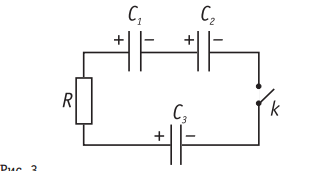
\includegraphics[scale=0.7]{115.png}  
\end{center}

  



\end{document}


%%% Local Variables: 
%%% mode: latex
%%% TeX-engine:xetex
%%% TeX-PDF-mode: t
%%% End:
